\documentclass[11pt]{book}
\usepackage[labelfont={bf}, margin=1cm]{caption}
\usepackage{titling, titlepic}

\usepackage[colorinlistoftodos, bordercolor=white, backgroundcolor=cyan]{todonotes}
\usepackage{booktabs, caption, subcaption}
\usepackage{hyperref, comment}
\usepackage{algpseudocode, algorithm}
\begin{document}
\graphicspath{{.}{../results}}

\chapter{Results}
\label{chap:results}
\section{Results of the First Quantitative Experiment}
\label{sec:firstquantitative}
Firstly we are going to discuss the results of the first quantitative experiment. One thing that is noticable in all results is that there are periods in which the number of pedestrians, especially in slow and fast wander, is steady, after which the number drops drastically. After a few steps the number goes up again. In sync with this behavior the number of pedestrians remaining idle stays low, and increases when the other behaviors drop. This is easily explained. Slow and fast wander are behaviors that exist of a single action. When this action has been executed, which takes a few steps, the token of the pedestrian moves out of the attached Petri net into its base place. In order to move this token, a slot and sink transition have to be fired. These transitions do not have an associated action. When there is no action available for the pedestrian, it executes the idle behavior. Especially at the start, this effect is very prominent. This is because all pedestrians start the simulation at exactly the same moment. All pedestrians executing the same actions or actions that take the same amount of time stay synchronous. After a few dozens of steps, the behavior has varied more and the pedestrians are not as synchronous any more in going back to the idle "action".

Another thing that we can notice is that there are more or less four actions that dominate simulation, namely \emph{slow wander}, \emph{fast wander}, \emph{go to goal}, and \emph{idle action}.
\todo[inline]{What happened to lean against pillar?} Behavior like going to the toilet and waiting for their friend (which are both part of the same going to the toilet behavior and Petri-net) are only done by one or two pedestrians at a time. This is completely as expected. The go-to-toilet situation is shared, which means that one Petri-net is attached to multiple pedestrian Petri-nets. The more dominant actions belong to situations that are not shared and are instantiated for every pedestrian that enters it. That means that the shared Petri nets are only instantiated once for every situation, while the ones that aren't shared are instantiated many times.

In figure \ref{fig:linear0to1goal1to0}, \ref{fig:sigmoid100_0_10_1_goal1to0} and \ref{fig:gaussian200_50_1_goal1to0} we see the results for having a linear goal utility function that decreases from 1 to 0 and the utility function for other behavior varying. Figure \ref{fig:linear0to1goal1to0} and \ref{fig:sigmoid100_0_10_1_goal1to0} look very similar. The simulation starts out with a large preference for slow wander behavior, which decreases while fast wander increases. After about 70 steps however, the gotogoal action starts to dominate the simulation, increasing at a fast pace. This makes the other actions decrease rapidly until pedestrians are either idle (because they have already reached their goal) or still going to their goal. When we look at figure \ref{fig:gaussian200_50_1_goal1to0} we see that almost all pedestrians go to the goal in the first dozen of steps. Fast wander and slow wander become completely overshadowed.

 
\todo[inline]{Describe utility functions in captions formally}


\begin{figure}[b]
\centering            
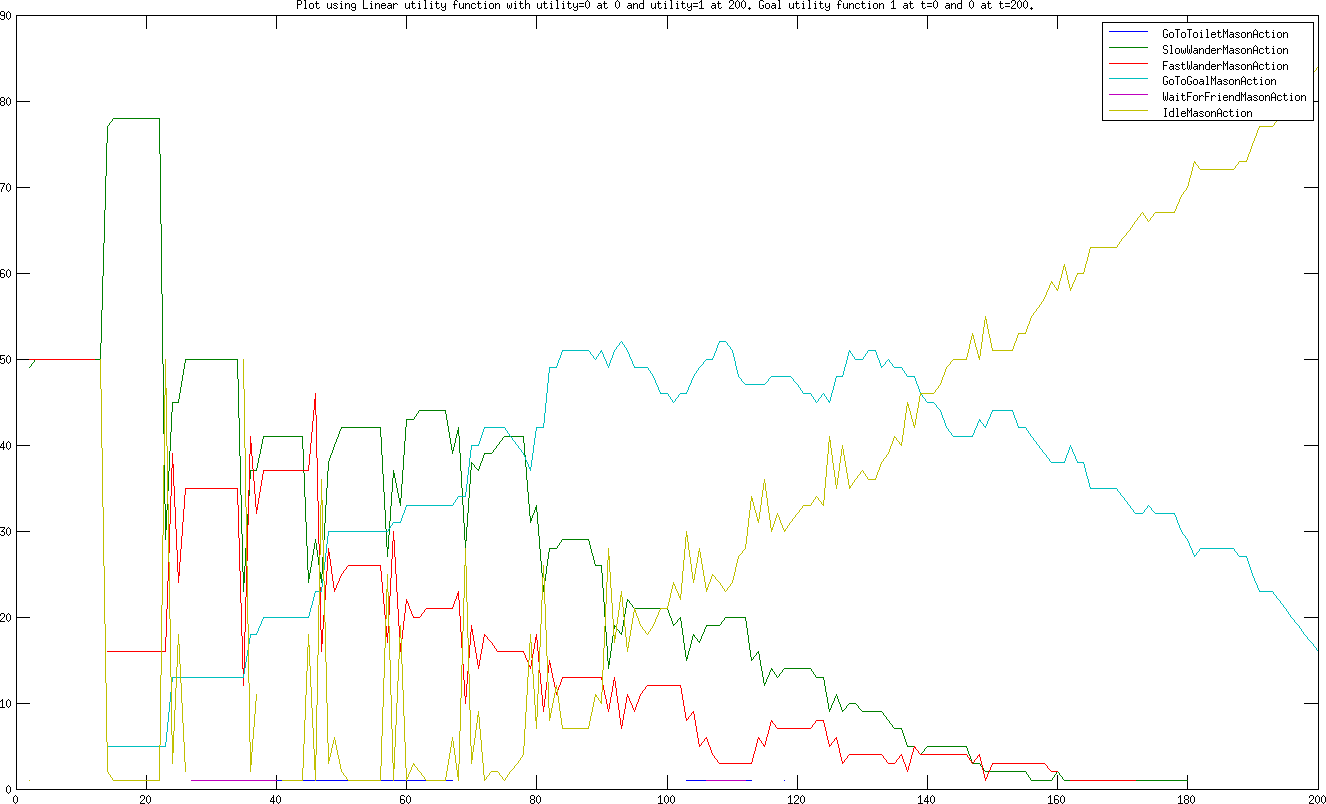
\includegraphics[width=\textwidth]{/home/djura/vakken/svn_afstudeerstage/deadline-driven-behavior/hulpscriptjes/goodresults/linear0to1goal1to0.png}
\caption{Goal utility linear with $U_0=1$ and $U_n = 0$. Other behavior utility linear with  $U_0=0$ and $U_n=1$.}
\label{fig:linear0to1goal1to0}
\end{figure}

\begin{figure}[b]
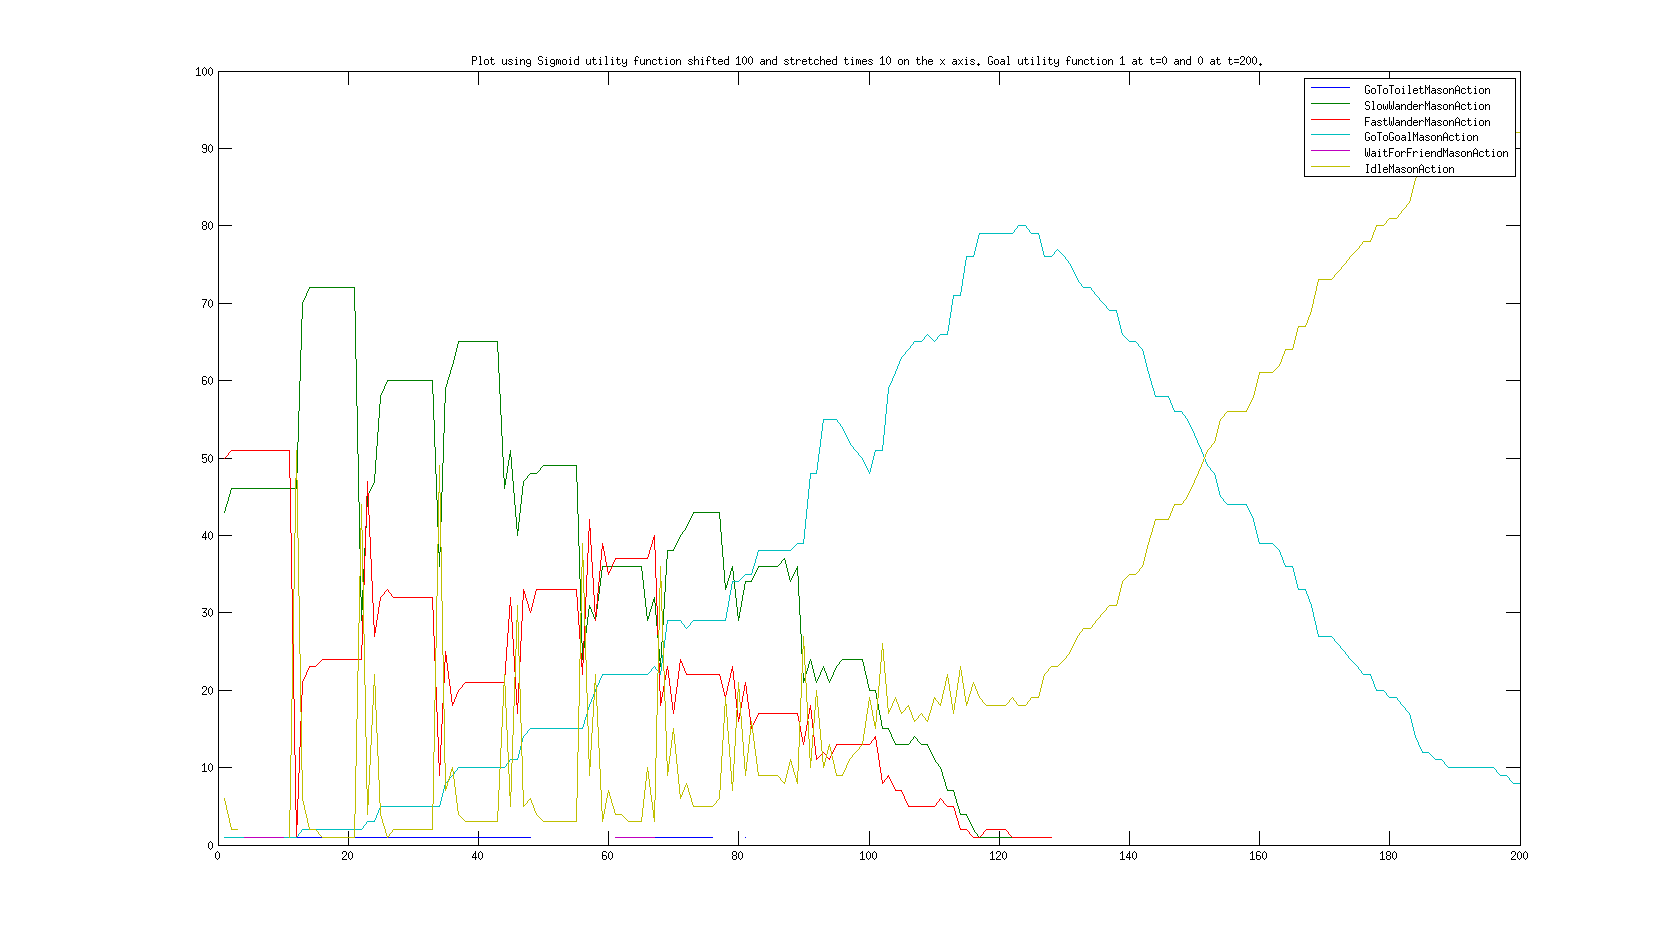
\includegraphics[width=\textwidth]{/home/djura/vakken/svn_afstudeerstage/deadline-driven-behavior/hulpscriptjes/goodresults/sigmoid100_0_10_1_goal1to0.png}
\caption{Goal utility linear with $U_0=1$ and $U_n = 0$. Other behavior utility function sigmoid100 0 10 1 goal1to0}
\label{fig:sigmoid100_0_10_1_goal1to0}
\end{figure}

\begin{figure}[b]
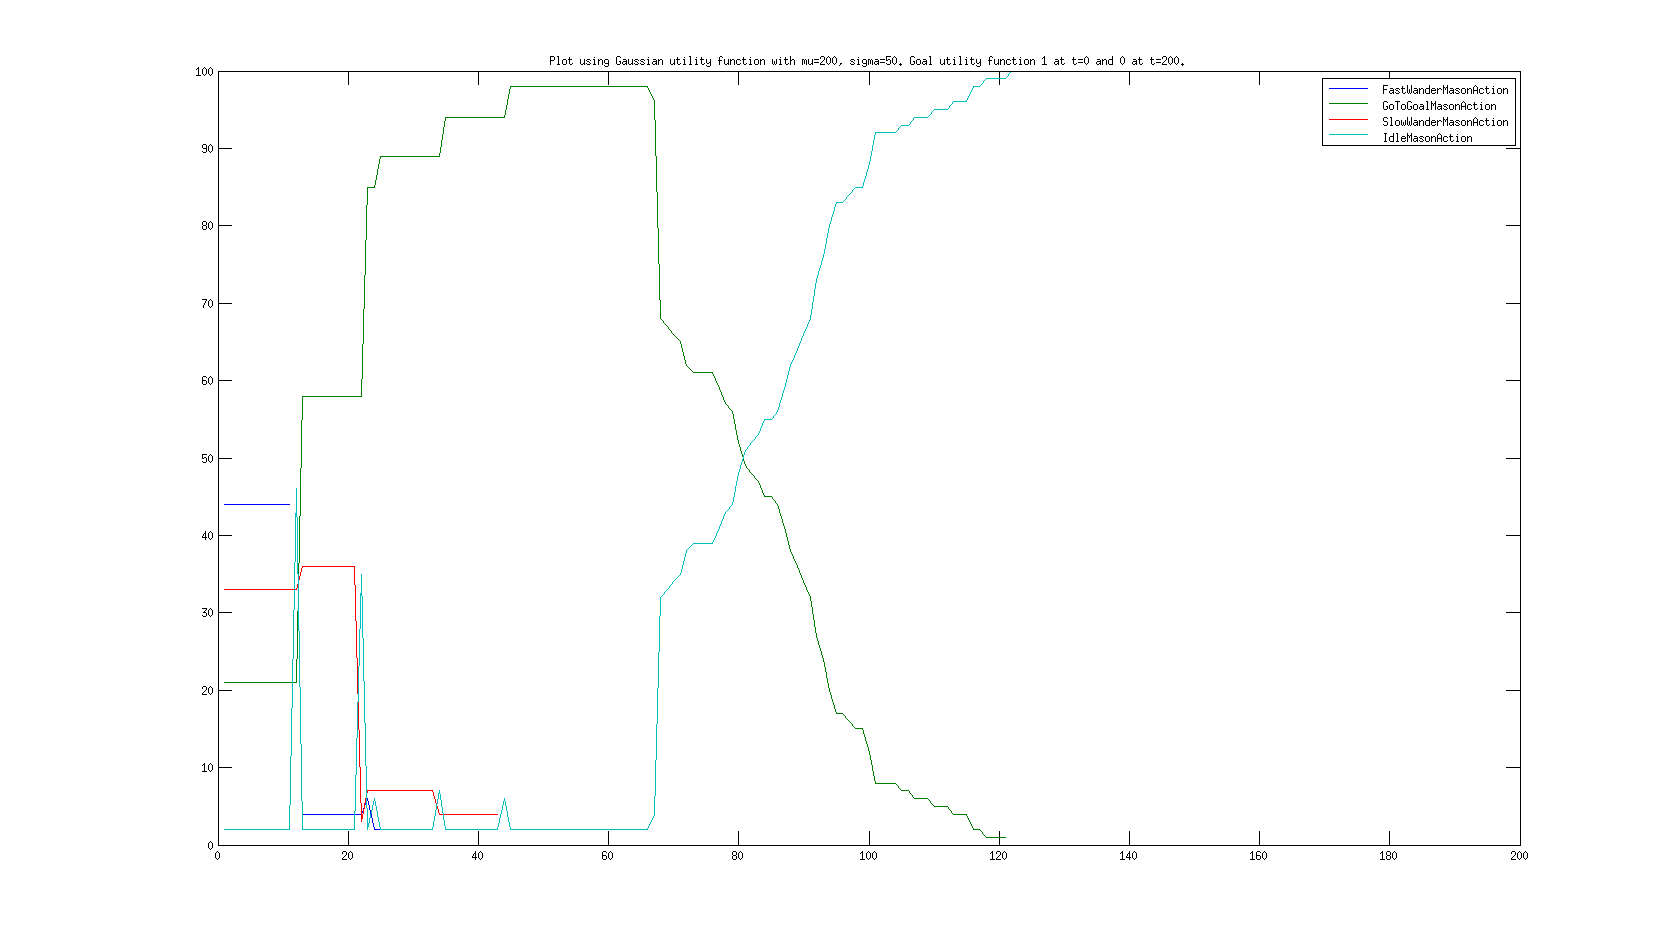
\includegraphics[width=\textwidth]{/home/djura/vakken/svn_afstudeerstage/deadline-driven-behavior/hulpscriptjes/goodresults/gaussian200_50_1_goal1to0.png}
\caption{gaussian200 50 1 goal1to0}
\label{fig:gaussian200_50_1_goal1to0}
\end{figure}


%%%%%%%%%%%%%%%%%%%%%%%%%%%%%%%%%%%%%%%%%%%%%%%%%%%%%%

In figures \ref{fig:linear0to1_goal01to0}, \ref{fig:sigmoid_100_0_10_1goal01to0} and \ref{fig:gaussian200_50_1_goal01to0} we see the results for the experiments with the goal utility function with $U_0=0.1$ and $U_n=0$. We varied the utility function of the other behavior the same as before. For some reason, the go-to-toilet and wait-for-friend actions are not present in this simulation. They have been replaced by the stand-still action. We would have expected to see more variation in actions now the utility of the go-to-goal behavior has been lowered. Instead, the time-consuming go-to-toilet behavior has been replaced by the less demanding stand-still behavior.

\begin{figure}
\centering
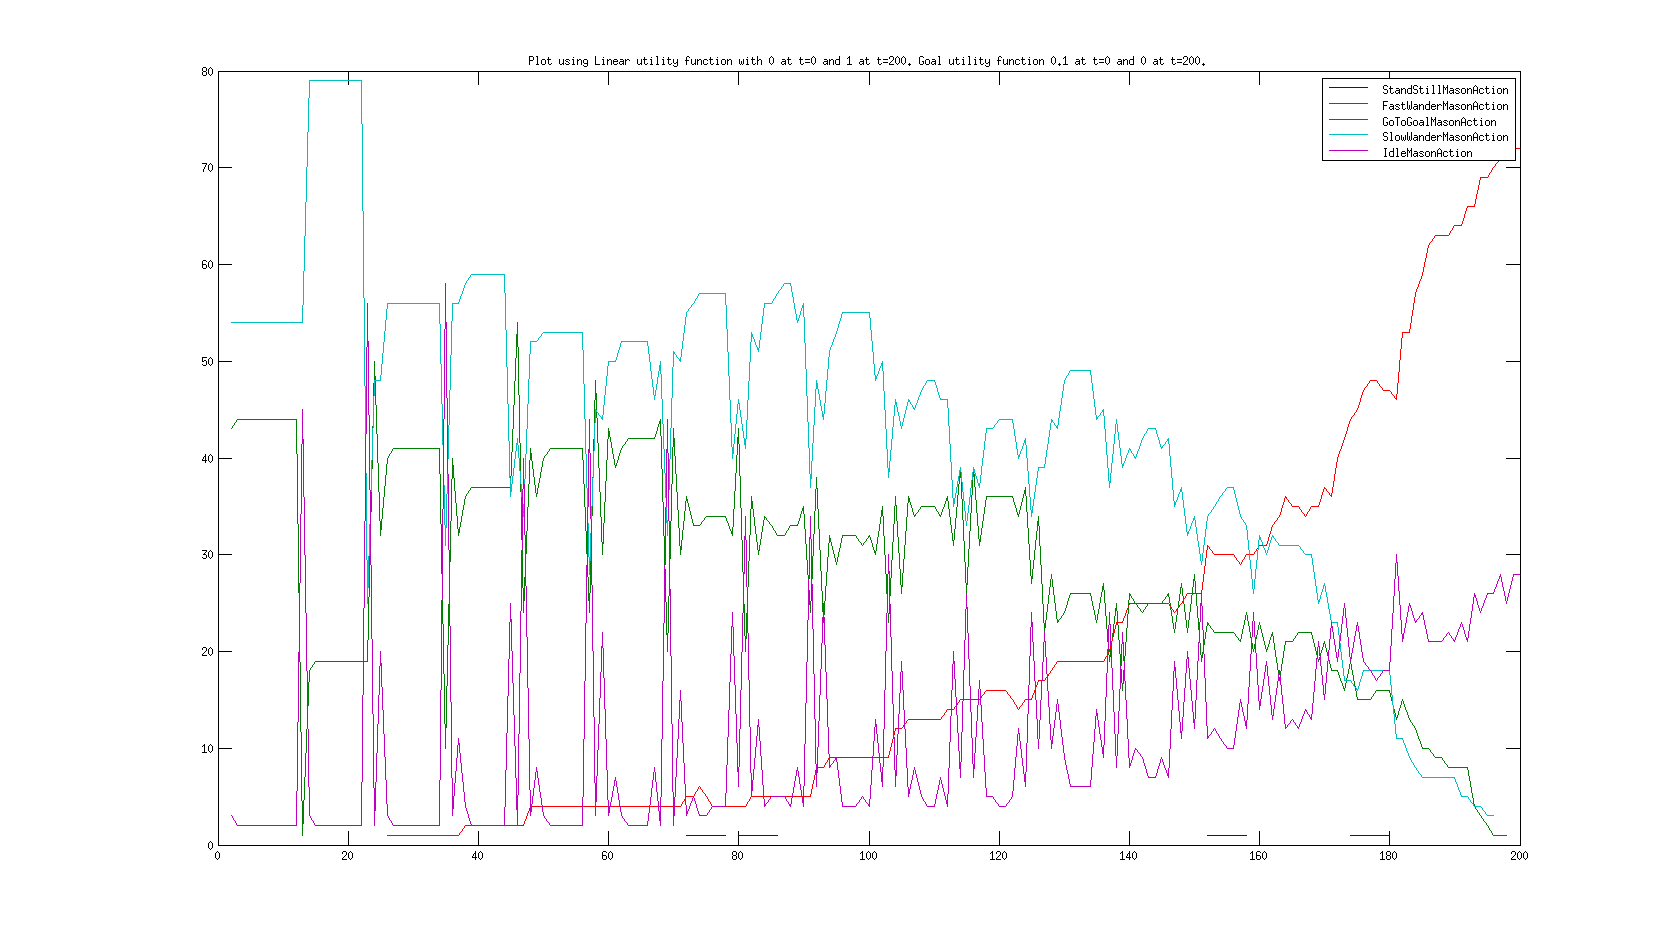
\includegraphics[width=\textwidth]{/home/djura/vakken/svn_afstudeerstage/deadline-driven-behavior/hulpscriptjes/goodresults/linear0to1_goal01to0.png}
\caption{linear0to1 goal01to0}
\label{fig:linear0to1_goal01to0}
\end{figure}

\begin{figure}
\centering
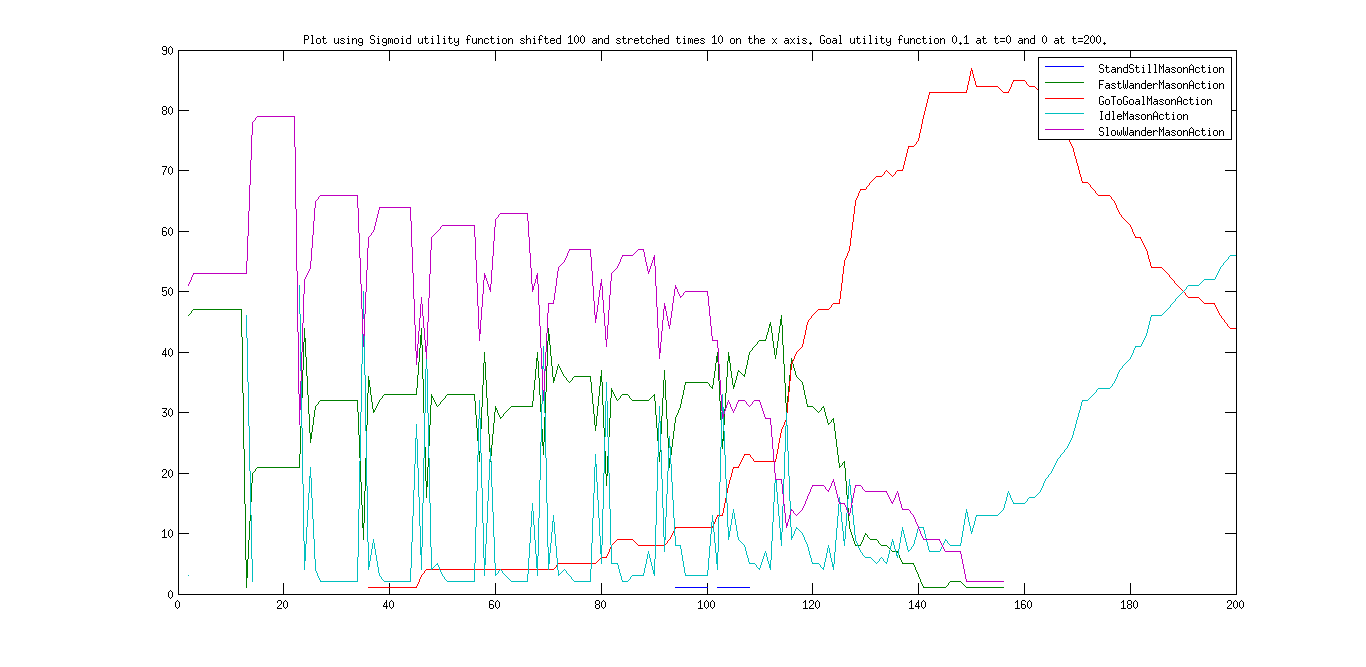
\includegraphics[width=\textwidth]{/home/djura/vakken/svn_afstudeerstage/deadline-driven-behavior/hulpscriptjes/goodresults/sigmoid_100_0_10_1goal01to0.png}
\caption{sigmoid 100 0 10 1 goal01to0}
\label{fig:sigmoid_100_0_10_1goal01to0}
\end{figure}

\begin{figure}
\centering
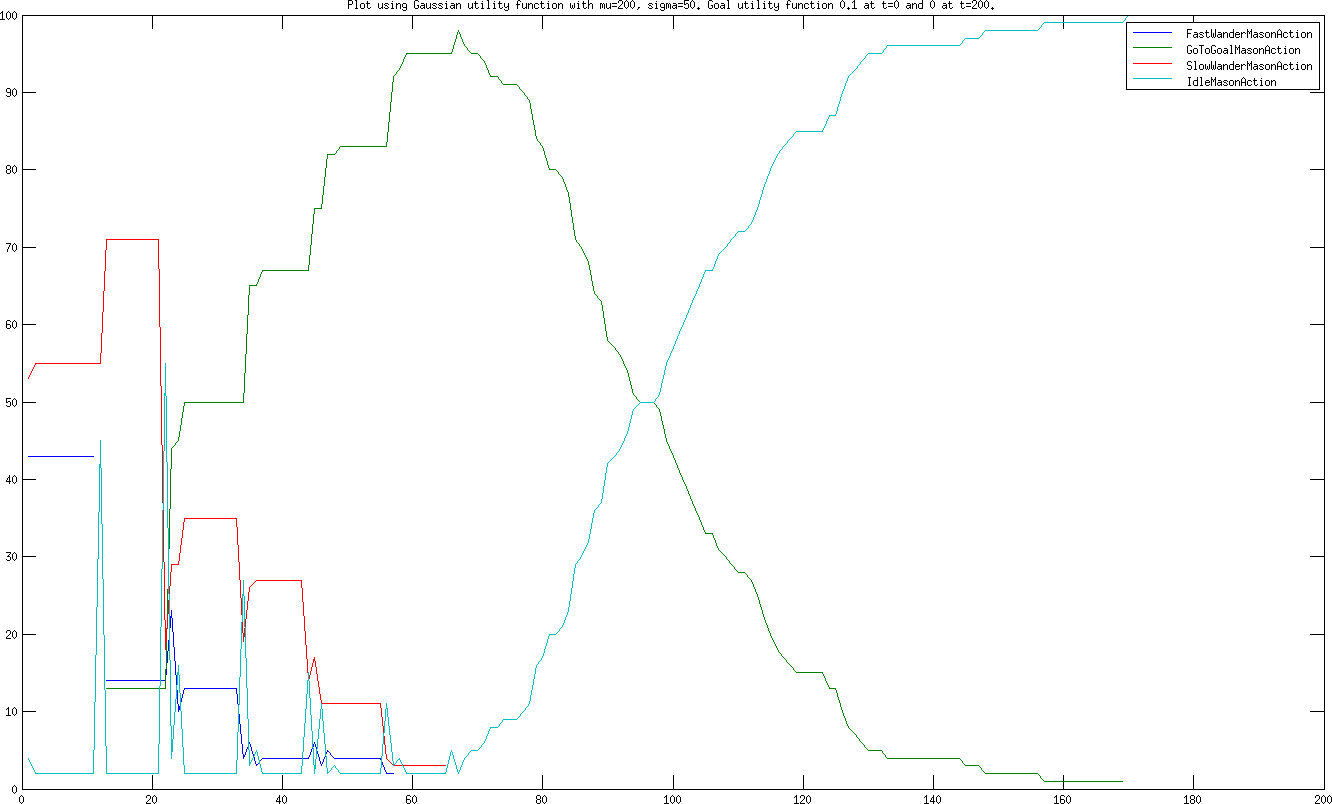
\includegraphics[width=\textwidth]{/home/djura/vakken/svn_afstudeerstage/deadline-driven-behavior/hulpscriptjes/goodresults/gaussian200_50_1_goal01to0.png}
\caption{gaussian200 50 1 goal01to0}
\label{fig:gaussian200_50_1_goal01to0}
\end{figure}

%%%%%%%%%%%%%%%%%%%%%%%%%%%%%%%%%%%%%%%%%%%%%%%%%%%%%%

In figure \ref{fig:linear0_1_200_goalsigmoid_100_0_-10_1}, \ref{fig:sigmoid100_0_10_1_goalsigmoid100_0_-10_1} and \ref{fig:gaussian200_50_1_goalsigmoid_100_0_-10_1} are the results for the experiments with a sigmoid goal utility function where $t_0=100$, $\beta=1$, $\omega=-10$ and $\eta=1$. The effects are more or less the same as for the previous results. Again, the sigmoid goal utility function causes the pedestrians to go to the goal very soon, eliminating the possibility to do other behavior very soon in the simulation.

\begin{figure}
\centering
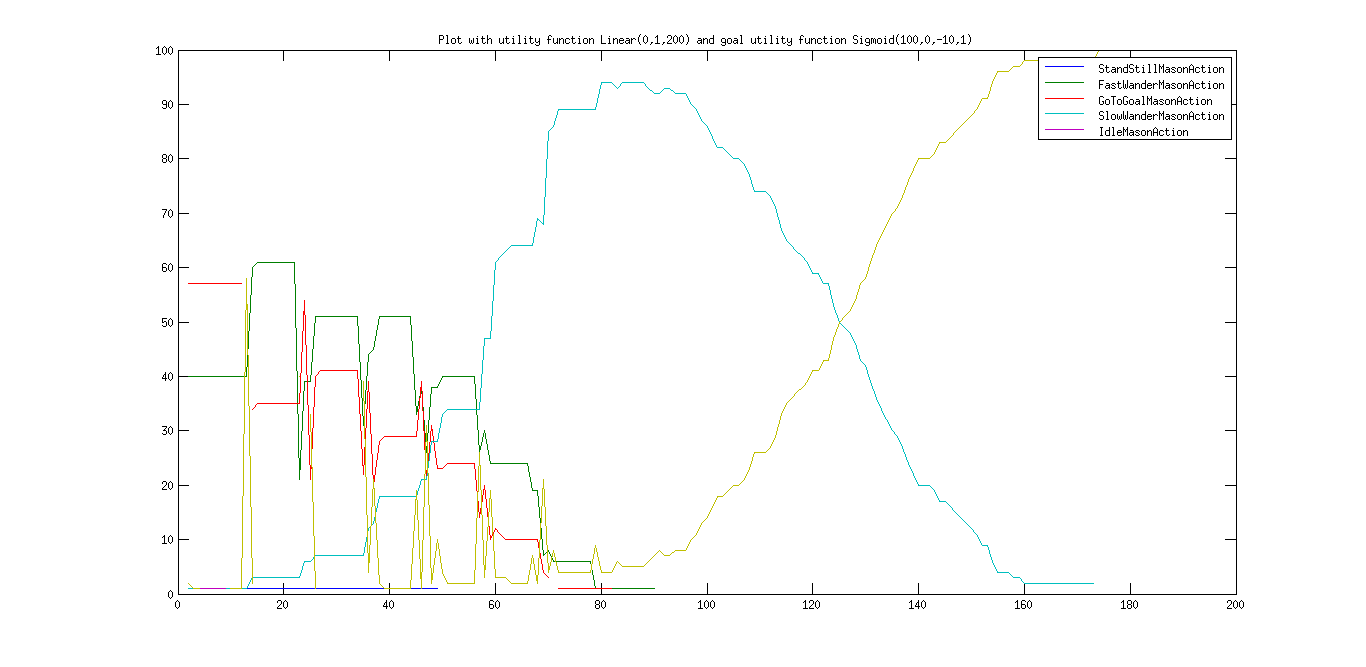
\includegraphics[width=\textwidth]{/home/djura/vakken/svn_afstudeerstage/deadline-driven-behavior/hulpscriptjes/goodresults/linear0_1_200_goalsigmoid_100_0_-10_1.png}
\caption{linear0 1 200 goalsigmoid 100 0 -10 1}
\label{fig:linear0_1_200_goalsigmoid_100_0_-10_1}
\end{figure}


\begin{figure}
\centering
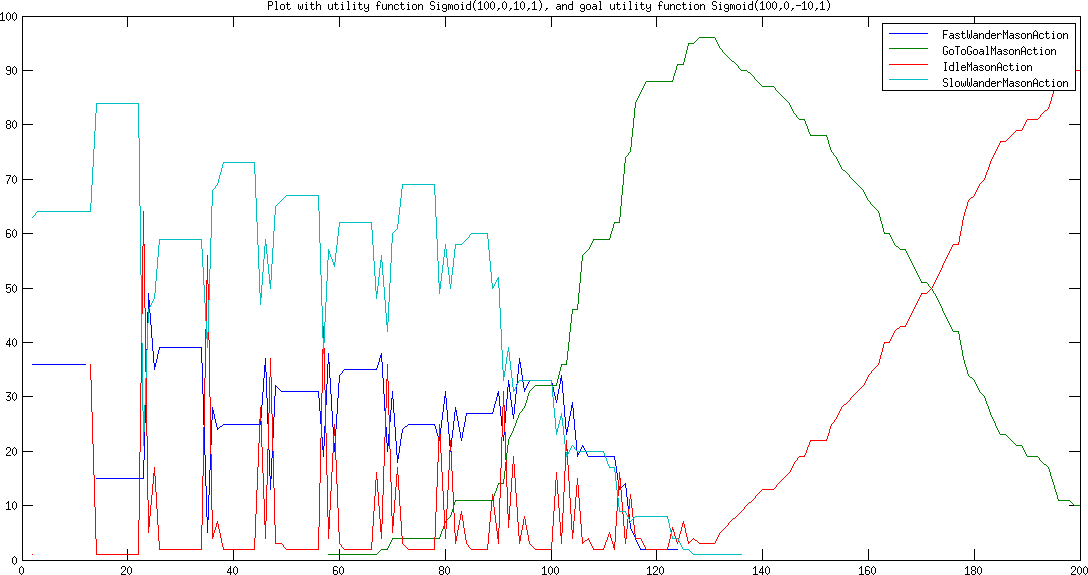
\includegraphics[width=\textwidth]{/home/djura/vakken/svn_afstudeerstage/deadline-driven-behavior/hulpscriptjes/goodresults/sigmoid100_0_10_1_goalsigmoid100_0_-10_1.png}
\caption{sigmoid100 0 10 1 goalsigmoid100 0 -10 1}
\label{fig:sigmoid100_0_10_1_goalsigmoid100_0_-10_1}
\end{figure}

\begin{figure}
\centering
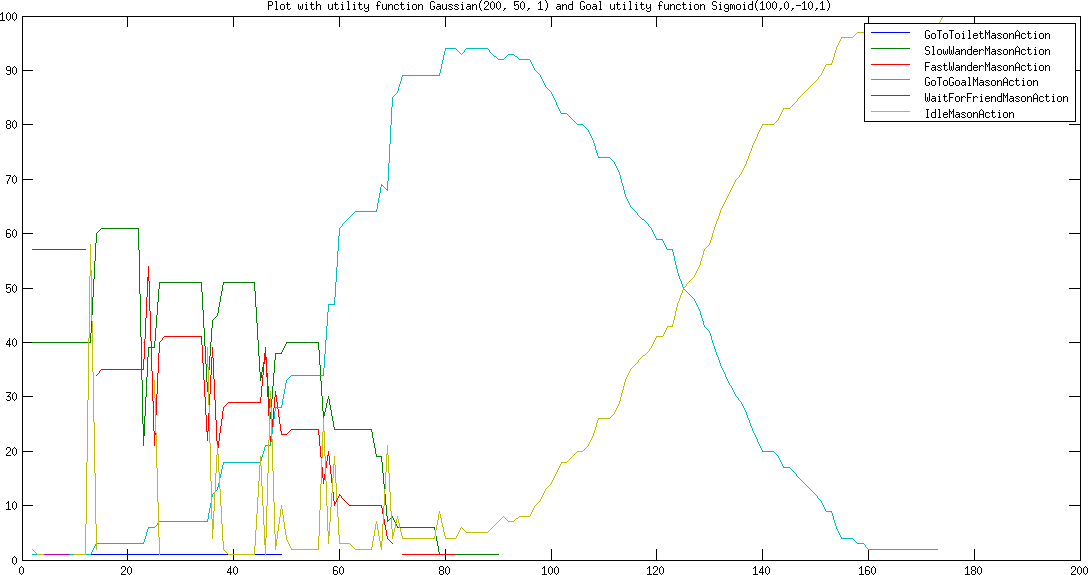
\includegraphics[width=\textwidth]{/home/djura/vakken/svn_afstudeerstage/deadline-driven-behavior/hulpscriptjes/goodresults/gaussian200_50_1_goalsigmoid_100_0_-1_1.png}
\caption{gaussian200 50 1 goalsigmoid 100 0 -10 1}
\label{fig:gaussian200_50_1_goalsigmoid_100_0_-10_1}
\end{figure}

The results for a Gaussian goal probability function are shown in figure \ref{fig:sigmoid100_0_10_1_goalgaussian0_50_1}, \ref{fig:linear0_1_200_goalgaussian_0_50_1} and \ref{fig:gaussian200_50_1_goalgaussian0_50_1}. We see that in general, the pedestrians seem to wait longer before they go to their goals. This also causes more pedestrians to be too late, because they still are on their way to the goal when the deadline passes. This is very likely due to the fact that the estimation of going to the goal is too low for some pedestrians, because the area they move in is larger than I took into account when estimating the time needed to go to the goal. \todo[inline]{Rerun these experiments with a more limited moving area?}.


\begin{figure}[h]
\centering
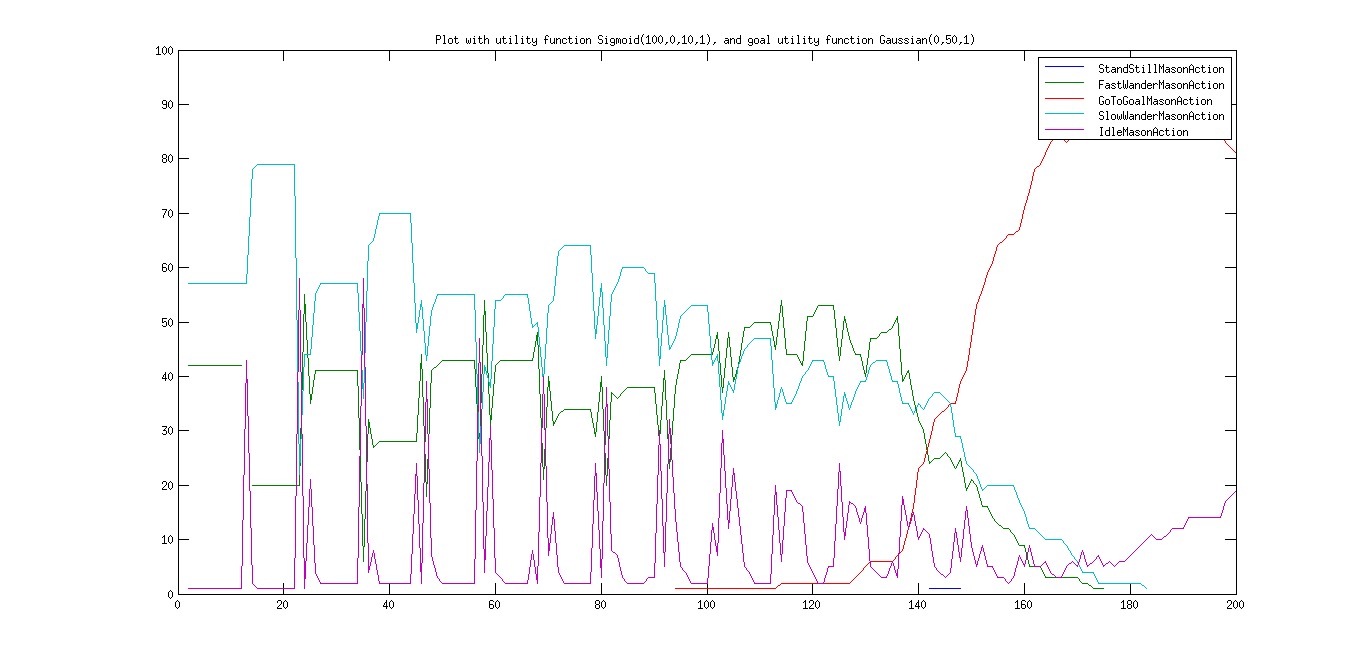
\includegraphics[width=\textwidth]{/home/djura/vakken/svn_afstudeerstage/deadline-driven-behavior/hulpscriptjes/goodresults/sigmoid100_0_10_1_goalgaussian0_50_1.png}
\caption{sigmoid100 0 10 1 goalgaussian0 50 1}
\label{fig:sigmoid100_0_10_1_goalgaussian0_50_1}
\end{figure}

\begin{figure}[h]
\centering
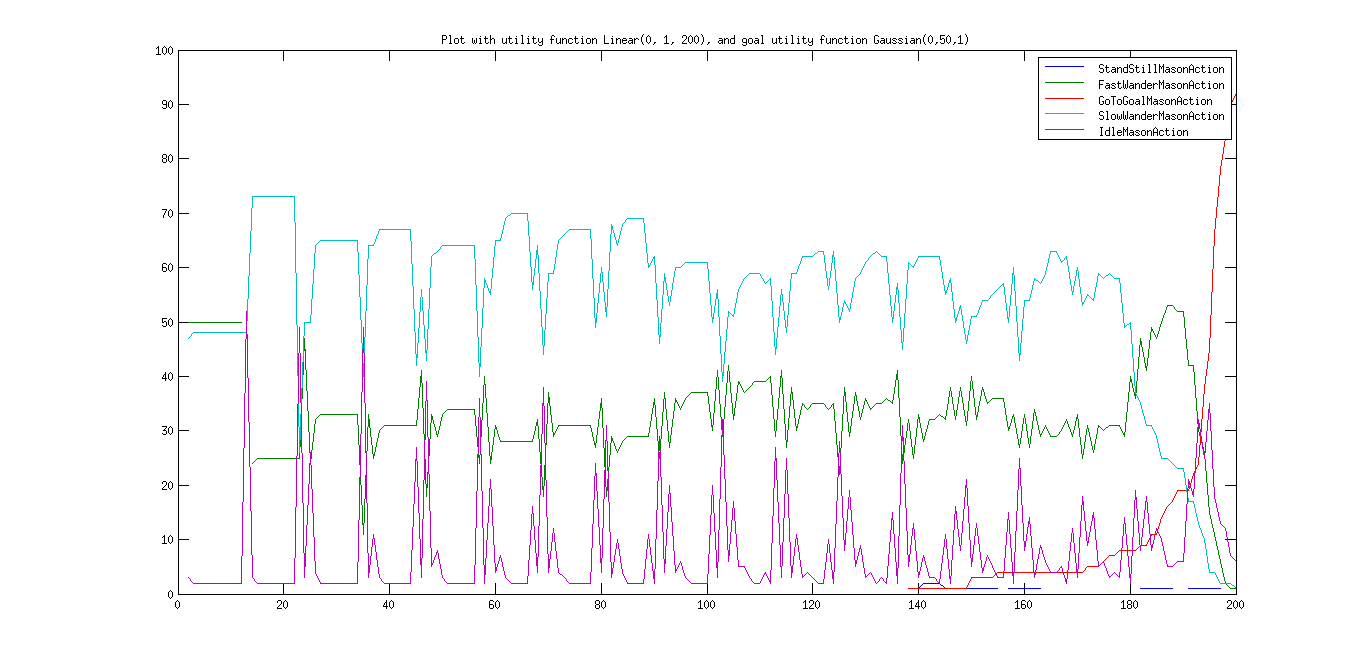
\includegraphics[width=\textwidth]{/home/djura/vakken/svn_afstudeerstage/deadline-driven-behavior/hulpscriptjes/goodresults/linear0_1_200_goalgaussian_0_50_1.png}
\caption{linear0 1 200 goalgaussian 0 50 1}
\label{fig:linear0_1_200_goalgaussian_0_50_1}
\end{figure}

\begin{figure}[h]
\centering
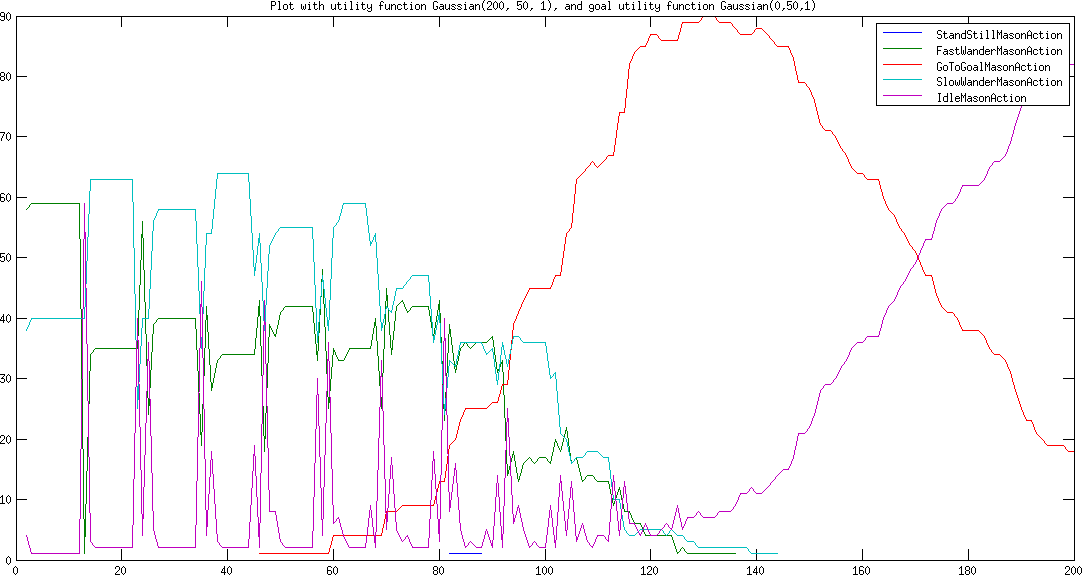
\includegraphics[width=\textwidth]{/home/djura/vakken/svn_afstudeerstage/deadline-driven-behavior/hulpscriptjes/goodresults/gaussian200_50_1_goalgaussian0_50_1.png}
\caption{gaussian200 50 1 goalgaussian0 50 1}
\label{fig:gaussian200_50_1_goalgaussian0_50_1}
\end{figure}

One problem we have with these results is that the number of pedestrians going to their goal goes up very fast from a certain point in time, regardless of the exact shape of the utility function. Consequently it is quite difficult to see if relaxed and hurried behavior actually emerges from our framework. This problem will be discussed in further detail in section \ref{chap:conclusiondiscusssion}. This was why we decided to do the second quantitative experiment that we described in the previous chapter (\ref{sec:quantitativeexp2}). The results can be found in section \ref{sec:secondquantitativeexperimentresults}.

\todo[inline]{What should I do with figure \ref{fig:linear0to1goal01}?}

\begin{figure}[h]
\centering
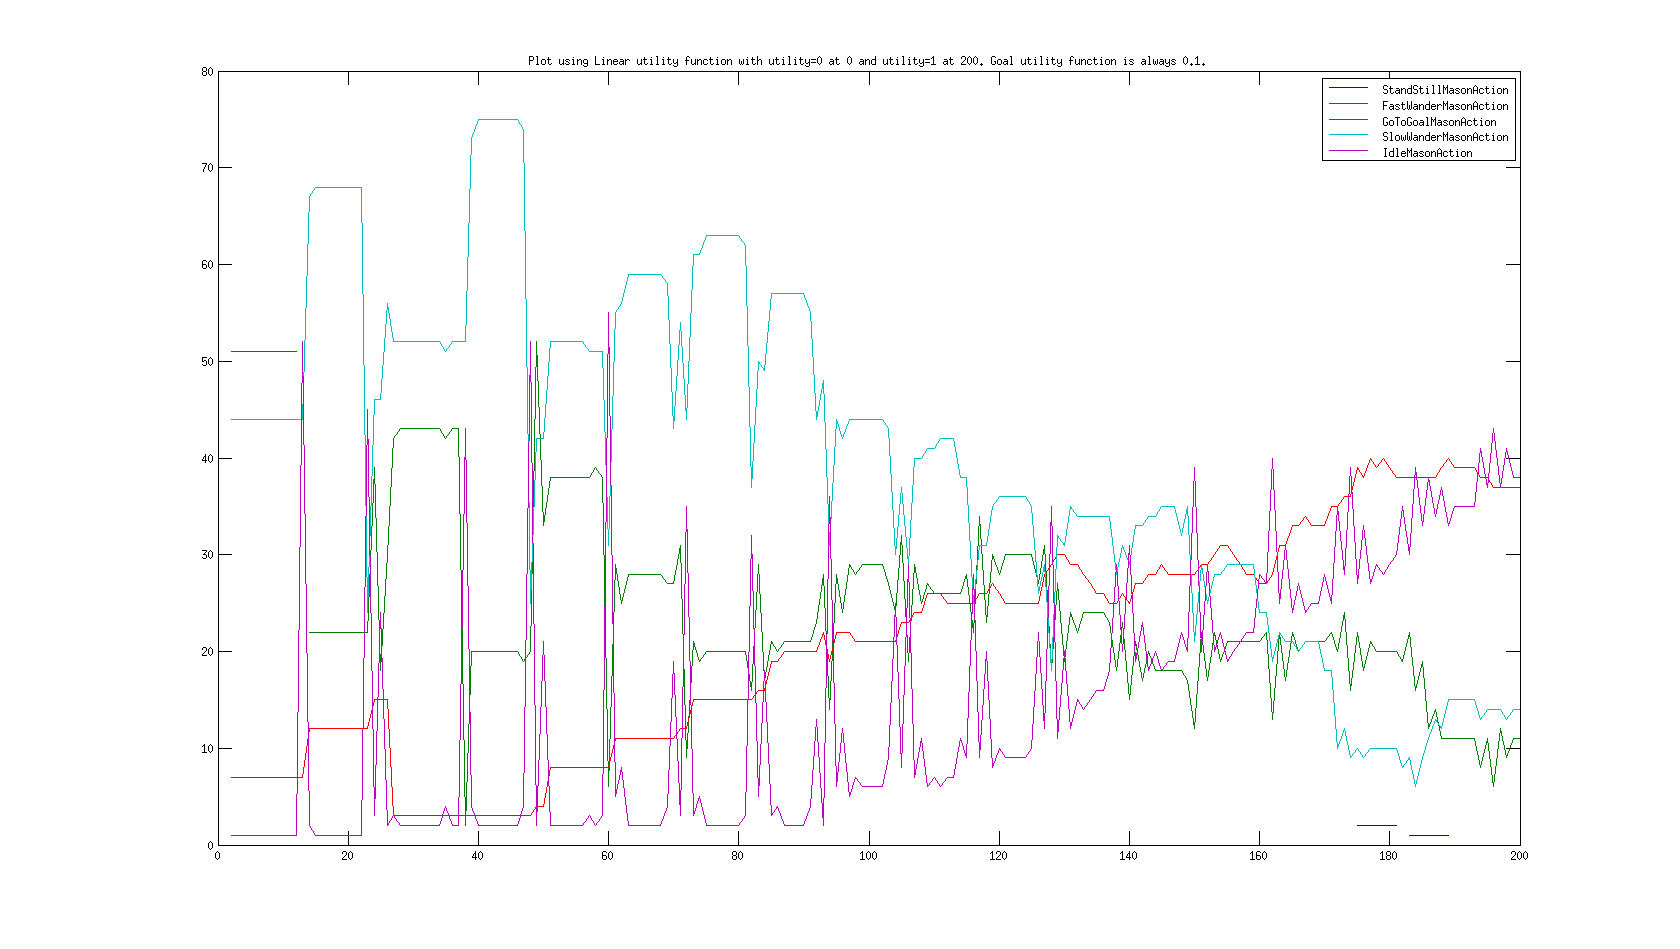
\includegraphics[width=\textwidth]{/home/djura/vakken/svn_afstudeerstage/deadline-driven-behavior/hulpscriptjes/goodresults/linear0to1goal01.png}
\caption{linear0to1goal01}
\label{fig:linear0to1goal01}
\end{figure}


\clearpage


%\section{Results for Sigmoid Function}
%
%
%\section{Results for Linear Function}
%It turns out a linear function gives significantly different behavior than a sigmoid function. Because there is a constant rise in the probability of walking to the goal, the pedestrians reach the goal very early, since there is a chance to go there every step, and this chance steadily increases. So all pedestrians have reached the goal long before the deadline. This is because the cumulative probability of the pedestrian going to the goal is very high very early.
%
%\section{Results for Gaussian Function}
%
%\section{Results}
%Below you will find the results of the quantitative experiment, where we used a variety of functions to check whether emergent behavior occurs.
%
%In figure \ref{result_toilet_linear_1_05_02_01_001}, you can see the results of choosing a linear function where the maximum is 0.001, 0.01, 0.02, 0.05 and 1.0 respectively as the goal probability function. We can see here that the pedestrians reach their goal very early, that is, 100 \% of the pedestrians reach the goal so early, they could easily have used the remaining time to do a multitude of other activities.
%
%\todo[inline]{Aggegrate graphs
%How am I going to aggegrate the graphs? }
%\begin{figure}
%\centering
%\includegraphics[width=280pt]{"/allautomaticresults/result_toilet_linear_1_05_02_01_001"}
%\caption{Blue: max = 1\\ green: max. = 0.5\\ red: max. = 0.2\\ turqooize: max. = 0.1\\ purple: max. = 0.01}
%\label{result_toilet_linear_1_05_02_01_001}
%\end{figure}
%
%In figure \ref{evaluation_log_linear0point5automatedpointcsv} the same effect can be seen even more exaggerated. Again, we see that the linear probability function causes the pedestrians to arrive at their goal far too early.
%
%\todo[inline]{Aggegrate graphs}
%\begin{figure}
%\centering
%\includegraphics[width=280pt]{"/allautomaticresults/result_toilet_linear_1_05_02_01_001"}
%\caption{Blue: max = 1\\ green: max. = 0.5\\ red: max. = 0.2\\ turqooize: max. = 0.1\\ purple: max. = 0.01}
%\label{result_toilet_linear_1_05_02_01_001}
%\end{figure}
%
%
%\begin{figure}
%\centering
%\includegraphics[width=250pt]{./automaticResults/evaluation_log_linear0point5automatedpointcsv.png}
%\caption{evaluation\_log\_linear0point5automatedpointcsv}
%\label{evaluation_log_linear0point5automatedpointcsv}
%\end{figure}
%
%\begin{figure}
%\centering
%\includegraphics[width=250pt]{./automaticResults/evaluation_log_linear1automatedpointcsv.png}
%%\caption{The global workings of our framework}
%\label{evaluation_log_linear1automatedpointcsv}
%\end{figure}
%
%
%
%In figure \ref{evaluation_log_sigmoid0point01automatedpointcsv} we see the results of using a sigmoid for goal probability function with a minimum \todo[inline]{find out how to describe, since those values only count in the limit or whatever} of 0 and a maximum of 0.01. Again we see that a maximum probability of 0.01 is low to have the pedestrians reach their goal in time.
%
%\begin{figure}
%\centering
%\includegraphics[width=250pt]{./automaticResults/evaluation_log_sigmoid0point01automatedpointcsv.png}
%\caption{evaluation\_log\_sigmoid0point01automatedpointcsv}
%\label{evaluation_log_sigmoid0point01automatedpointcsv}
%\end{figure}
%
%
%
%\begin{figure}
%\centering
%\includegraphics[width=250pt]{./automaticResults/evaluation_log_sigmoid0point1automatedpointcsv.png}
%%\caption{The global workings of our framework}
%caption{evaluation\_log\_sigmoid0point1automatedpointcsv}
%\label{evaluation_log_sigmoid0point1automatedpointcsv}
%\end{figure}
%
%\begin{figure}
%\centering
%\includegraphics[width=250pt]{./automaticResults/evaluation_log_sigmoid0point2automatedpointcsv.png}
%%\caption{The global workings of our framework}
%\caption{evaluation\_log\_sigmoid0point2automatedpointcsv}
%\label{evaluation_log_sigmoid0point2automatedpointcsv}
%\end{figure}
%
%\begin{figure}
%\centering
%\includegraphics[width=250pt]{./automaticResults/evaluation_log_sigmoid0point5automatedpointcsv.png}
%%\caption{The global workings of our framework}
%\caption{evaluation\_log\_sigmoid0point5automatedpointcsv}
%\label{evaluation_log_sigmoid0point5automatedpointcsv}
%\end{figure}
%
%We can only say more about the results if the frequencies are divided by the total number of pedestrians in the simulation at that moment. The curve we see in figure \ref{evaluation_log_sigmoid0point01automatedpointcsv}, \ref{evaluation_log_sigmoid0point1automatedpointcsv}, \ref{evaluation_log_sigmoid0point2automatedpointcsv}, and \ref{evaluation_log_sigmoid0point5automatedpointcsv} (though to a lesser extent) can be explained by a multitude of causes. First of all, it can be explained by the fact that the number of pedestrians in the simulation diminishes as they finish their goal action. It could also be caused by the probability function increasing, but in this case, that is highly unlikely, because that would result in data quite opposite to the results here. Lastly, it could be that at certain moments, there are more pedestrians already engaged in other multi-step activities.
%
%
%\section{Results 2}
%Below follow the results of the other actions, that is, the actions that are not directly connected to the goal probability. The results of these actions have to show that our framework is also capable of generating \emph{emergent} behavior.
%
%\todo[inline]{Merge results that were accidentally separated}
%
%%\begin{figure}
%%\centering
%%\includegraphics[width=250pt]{./automaticResults2/evaluation_log2_gaussian0point01twoPeopleToiletSituationpointxmlpointcsv.png}
%%%\caption{The global workings of our framework}
%%\label{evaluation_log2_gaussian0point01twoPeopleToiletSituationpointxmlpointcsv}
%%\end{figure}
%%
%%\begin{figure}
%%\centering
%%\includegraphics[width=250pt]{./automaticResults2/evaluation_log2_gaussian0point2pillarSituationpointxmlpointcsv.png}
%%%\caption{The global workings of our framework}
%%\label{evaluation_log2_gaussian0point2pillarSituationpointxmlpointcsv}
%%\end{figure}
%%
%%\begin{figure}
%%\centering
%%\includegraphics[width=250pt]{./automaticResults2/evaluation_log2_gaussian0point2standStillSituationpointxmlpointcsv.png}
%%%\caption{The global workings of our framework}
%%\label{evaluation_log2_gaussian0point2standStillSituationpointxmlpointcsv}
%%\end{figure}
%%
%%\todo[inline]{This graph was probably made for the toilet situation that is now saved as twopeopletoiletsituation.xml, but the design of the petrinet is possibly flawed, and could maybe better be replaced by twopeopletoiletsituation2.xml. What also possibly is missing is that the pedestrian could maybe come back after having gone to the toilet.}
%%\begin{figure}
%%\centering
%%\includegraphics[width=250pt]{./automaticResults2/evaluation_log2_gaussian0point2twoPeopleToiletSituationpointxmlpointcsv.png}
%%%\caption{The global workings of our framework}
%%\label{evaluation_log2_gaussian0point2twoPeopleToiletSituationpointxmlpointcsv}
%%\end{figure}
%%
%%\begin{figure}
%%\centering
%%\includegraphics[width=250pt]{./automaticResults2/evaluation_log2_gaussian0point5pillarSituationpointxmlpointcsv.png}
%%%\caption{The global workings of our framework}
%%\label{evaluation_log2_gaussian0point5pillarSituationpointxmlpointcsv}
%%\end{figure}
%%
%%\begin{figure}
%%\centering
%%\includegraphics[width=250pt]{./automaticResults2/evaluation_log2_gaussian0point5standStillSituationpointxmlpointcsv.png}
%%%\caption{The global workings of our framework}
%%\label{evaluation_log2_gaussian0point5standStillSituationpointxmlpointcsv}
%%\end{figure}
%%
%%\begin{figure}
%%\centering
%%\includegraphics[width=250pt]{./automaticResults2/evaluation_log2_gaussian0point5twoPeopleToiletSituationpointxmlpointcsv.png}
%%%\caption{The global workings of our framework}
%%\label{evaluation_log2_gaussian0point5twoPeopleToiletSituationpointxmlpointcsv}
%%\end{figure}
%%
%%\begin{figure}
%%\centering
%%\includegraphics[width=250pt]{./automaticResults2/evaluation_log2_linear0point01automated-pillarSituationpointcsv.png}
%%%\caption{The global workings of our framework}
%%\label{evaluation_log2_linear0point01automated-pillarSituationpointcsv}
%%\end{figure}
%%\clearpage
%%
%%\begin{figure}
%%\centering
%%\includegraphics[width=250pt]{./automaticResults2/evaluation_log2_linear0point01automated-standStillSituationpointcsv.png}
%%%\caption{The global workings of our framework}
%%\label{evaluation_log2_linear0point01automated-standStillSituationpointcsv}
%%\end{figure}
%%
%%\begin{figure}
%%\centering
%%\includegraphics[width=250pt]{./automaticResults2/evaluation_log2_linear0point01automated-twoPeopleToiletSituationpointcsv.png}
%%%\caption{The global workings of our framework}
%%\label{evaluation_log2_linear0point01automated-twoPeopleToiletSituationpointcsv}
%%\end{figure}
%%
%%\begin{figure}
%%\centering
%%\includegraphics[width=250pt]{./automaticResults2/evaluation_log2_linear0point1automated-standStillSituationpointcsv.png}
%%%\caption{The global workings of our framework}
%%\label{evaluation_log2_linear0point1automated-standStillSituationpointcsv}
%%\end{figure}
%%
%%\begin{figure}
%%\centering
%%\includegraphics[width=250pt]{./automaticResults2/evaluation_log2_linear0point1automated-twoPeopleToiletSituationpointcsv.png}
%%%\caption{The global workings of our framework}
%%\label{evaluation_log2_linear0point1automated-twoPeopleToiletSituationpointcsv}
%%\end{figure}
%%
%%\begin{figure}
%%\centering
%%\includegraphics[width=250pt]{./automaticResults2/evaluation_log2_linear0point2automatedstandStillSituationpointxmlpointcsv.png}
%%%\caption{The global workings of our framework}
%%\label{evaluation_log2_linear0point2automatedstandStillSituationpointxmlpointcsv}
%%\end{figure}
%%
%%\begin{figure}
%%\centering
%%\includegraphics[width=250pt]{./automaticResults2/evaluation_log2_linear0point2automatedtwoPeopleToiletSituationpointxmlpointcsv.png}
%%%\caption{The global workings of our framework}
%%\label{evaluation_log2_linear0point2automatedtwoPeopleToiletSituationpointxmlpointcsv}
%%\end{figure}
%%\clearpage
%%
%%\begin{figure}
%%\centering
%%\includegraphics[width=250pt]{./automaticResults2/evaluation_log2_linear0point5automatedtwoPeopleToiletSituationpointxmlpointcsv.png}
%%%\caption{The global workings of our framework}
%%\label{evaluatituation}
%%\end{figure}
%%
%%\begin{figure}
%%\centering
%%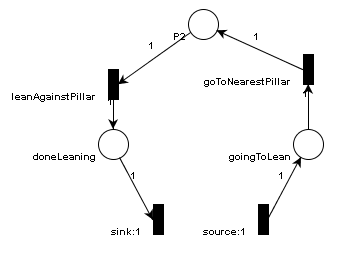
\includegraphics[width=250pt]{pillarSituation}
%%\caption{Behavior model for the pillar situation}
%%\label{pillarsituation}
%%\end{figure}ion_log2_linear0point5automatedtwoPeopleToiletSituationpointxmlpointcsv}
%%\end{figure}
%%
%%\begin{figure}
%%\centering
%%\includegraphics[width=250pt]{./automaticResults2/evaluation_log2_linear1automatedtwoPeopleToiletSituationpointxmlpointcsv.png}
%%%\caption{The global workings of our framework}
%%\label{evaluation_log2_linear1automatedtwoPeopleToiletSituationpointxmlpointcsv}
%%\end{figure}
%%
%%\begin{figure}
%%\centering
%%\includegraphics[width=250pt]{./automaticResults2/evaluation_log2_sigmoid0point01automatedpillarSituationpointxmlpointcsv.png}
%%%\caption{The global workings of our framework}
%%\label{evaluation_log2_sigmoid0point01automatedpillarSituationpointxmlpointcsv}
%%\end{figure}
%%
%%\begin{figure}
%%\centering
%%\includegraphics[width=250pt]{./automaticResults2/evaluation_log2_sigmoid0point01automatedstandStillSituationpointxmlpointcsv.png}
%%%\caption{The global workings of our framework}
%%\label{evaluation_log2_sigmoid0point01automatedstandStillSituationpointxmlpointcsv}
%%\end{figure}
%%
%%\begin{figure}
%%\centering
%%\includegraphics[width=250pt]{./automaticResults2/evaluation_log2_sigmoid0point01automatedtwoPeopleToiletSituationpointxmlpointcsv.png}
%%%\caption{The global workings of our framework}
%%\label{evaluation_log2_sigmoid0point01automatedtwoPeopleToiletSituationpointxmlpointcsv}
%%\end{figure}
%%
%%\begin{figure}
%%\centering
%%\includegraphics[width=250pt]{./automaticResults2/evaluation_log2sigmoid0point1automatedpillarSituationpointxmlpointcsv.png}
%%%\caption{The global workings of our framework}
%%\label{evaluation_log2sigmoid0point1automatedpillarSituationpointxmlpointcsv}
%%\end{figure}
%%
%%\begin{figure}
%%\centering
%%\includegraphics[width=250pt]{./automaticResults2/evaluation_log2sigmoid0point1automatedstandStillSituationpointxmlpointcsv.png}
%%%\caption{The global workings of our framework}
%%\label{evaluation_log2sigmoid0point1automatedstandStillSituationpointxmlpointcsv}
%%\end{figure}
%%\clearpage
%%
%%\begin{figure}
%%\centering
%%\includegraphics[width=250pt]{./automaticResults2/evaluation_log2sigmoid0point1automatedtwoPeopleToiletSituationpointxmlpointcsv.png}
%%%\caption{The global workings of our framework}
%%\label{evaluation_log2sigmoid0point1automatedtwoPeopleToiletSituationpointxmlpointcsv}
%%\end{figure}
%%
%%\begin{figure}
%%\centering
%%\includegraphics[width=250pt]{./automaticResults2/evaluation_log2sigmoid0point5automatedpillarSituationpointxmlpointcsv.png}
%%%\caption{The global workings of our framework}
%%\label{evaluation_log2sigmoid0point5automatedpillarSituationpointxmlpointcsv}
%%\end{figure}
%%
%%\begin{figure}
%%\centering
%%\includegraphics[width=250pt]{./automaticResults2/evaluation_log2sigmoid0point5automatedstandStillSituationpointxmlpointcsv.png}
%%%\caption{The global workings of our framework}
%%\label{evaluation_log2sigmoid0point5automatedstandStillSituationpointxmlpointcsv}
%%\end{figure}
%%\clearpage
%%
%%\begin{figure}
%%\centering
%%\includegraphics[width=250pt]{./automaticResults2/evaluation_log2sigmoid0point5automatedtwoPeopleToiletSituationpointxmlpointcsv.png}
%%%\caption{The global workings of our framework}
%%\label{evaluation_log2sigmoid0point5automatedtwoPeopleToiletSituationpointxmlpointcsv}
%%\end{figure}
%%
%%\begin{figure}
%%\centering
%%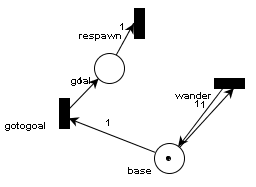
\includegraphics[width=200pt]{rotterdamPedestrianNet}
%%\caption{The basic petrinet for the pedestrian model for Rotterdam airport}
%%\label{basicnet}
%%\end{figure}
%%
%%\begin{figure}
%%\centering
%%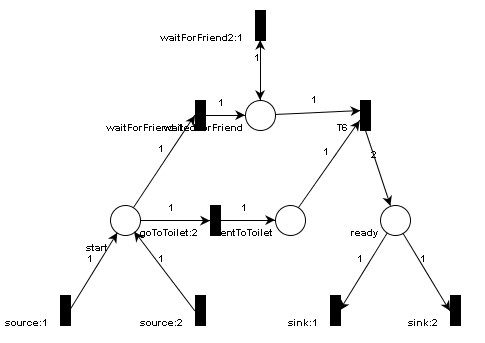
\includegraphics[width=350pt]{twoPeopleToiletSituation}
%%\caption{Behavior model for the toilet situation}
%%\label{toiletsituation}
%%\end{figure}
%%
%%\begin{figure}
%%\centering
%%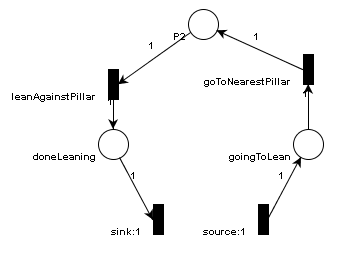
\includegraphics[width=250pt]{pillarSituation}
%%\caption{Behavior model for the pillar situation}
%%\label{pillarsituation}
%%\end{figure}

\section{Result of the Qualitative Experiment}
\todo[inline]{At this place there was previously a lot of stuff that I now commented out. Decide what to do with it. I shouldn´t put the missing graphs in my thesis in this form. Check if there is still useful stuff in there.}


%\section{What can we derive from these results?}
%From these results, we can see that not only does the changing of the goal probability function affect the time at which the agents decide when to %move to the goal, but also the time at which other actions are executed. This shows that our framework is able to generate emergent behavior. When %the probability of going to the goal is high, actions that take longer to finish have a very low frequency.

\section{Results of the Second Quantitative experiments}
\label{sec:secondquantitativeexperimentresults}
\todo[inline]{Check if I have to experiment with more parameters, e.g. with the Gaussian function}
\todo[inline]{Maybe regenerate the graphs so the text is larger, or find a different solution so the graphs can be more nicely positioned}
In the first experiment, the go-to-goal behavior was so dominant that it was difficult judge other emergent behavior. The following results will give a clearer view of whether hurried and relaxed behavior can emerge from our framework.

First of all, we have figure \ref{fig:constant1} where the $U=1$ for all $t$. We see the typical phases that we saw in section \ref{sec:firstquantitative} where most pedestrians execute slow- or fast wander for a while, after which the frequency of idle behavior goes up for a few steps. We can also see a few pedestrians doing the go-to-toilet and the accompanying wait-for-friend action. The frequencies of the actions deviate more or less around the same value through the whole simulation.

\begin{figure}
\centering
\includegraphics[width=\textwidth]{/home/djura/vakken/svn_afstudeerstage/deadline-driven-behavior/hulpscriptjes/goodresults/constant1_cropped}
\caption{constant1}
\label{fig:constant1}
\end{figure}

Next, we have the results for the utility functions that do decrease when time runs out. It is very clear that eliminating the goal gives the pedestrians the freedom to do different kinds of behavior. We see that the slow wander action has the preference most of the time, except when time has almost run out. Slow wander then decreases while fast wander increases, until even this less time consuming action takes too much time, and the pedestrians become idle. This preference of relaxed behavior (slow wander) until that takes to long to catch a deadline and transitioning to hurried behavior (fast wander) is exactly what we wanted to show with our framework.

We see that using a linear function with a lower maximum value gives the same effect as a linear function that has 1 as highest value (fig \ref{fig:linear0to1_100agents}, \ref{fig:linear0to0.5_100agents} and \ref{fig:linear0to1_100agents}. \todo[inline]{explain}

\todo[inline]{Do we need all these graphs?}

\begin{figure}
\centering
\includegraphics[width=\textwidth]{/home/djura/vakken/svn_afstudeerstage/deadline-driven-behavior/hulpscriptjes/goodresults/linear0to1_100agents.png}
\caption{linear0to1 100agents}
\label{fig:linear0to1_100agents}
\end{figure}


\begin{figure}
\centering
\includegraphics[width=\textwidth]{/home/djura/vakken/svn_afstudeerstage/deadline-driven-behavior/hulpscriptjes/goodresults/linear0to05_100agents.png}
\caption{linear0to 0.5 100agents}
\label{fig:linear0to0.5_100agents}
\end{figure}

\begin{figure}
\centering
\includegraphics[width=\textwidth]{/home/djura/vakken/svn_afstudeerstage/deadline-driven-behavior/hulpscriptjes/goodresults/linear0to01_100agents.png}
\caption{linear0to0.1 100agents}
\label{fig:linear0to1_100agents}
\end{figure}

\begin{figure}
\centering
\includegraphics[width=\textwidth]{/home/djura/vakken/svn_afstudeerstage/deadline-driven-behavior/hulpscriptjes/goodresults/sigmoidnotmultiplied_100agents.png}
\caption{sigmoidnotmultiplied 100agents (but shifted to the right}
\label{fig:sigmoidnotmultiplied_100agents}
\end{figure}

\begin{figure}
\centering
\includegraphics[width=\textwidth]{/home/djura/vakken/svn_afstudeerstage/deadline-driven-behavior/hulpscriptjes/goodresults/sigmoid xtimes20.png}
\caption{sigmoid xtimes20}
\label{fig:sigmoid xtimes20}
\end{figure}

\begin{figure}
\centering
\includegraphics[width=\textwidth]{/home/djura/vakken/svn_afstudeerstage/deadline-driven-behavior/hulpscriptjes/goodresults/sigmoid xtimes100.png}
\caption{sigmoid xtimes100}
\label{fig:sigmoid xtimes100}
\end{figure}

\begin{figure}
\centering
\includegraphics[width=\textwidth]{/home/djura/vakken/svn_afstudeerstage/deadline-driven-behavior/hulpscriptjes/goodresults/sigmoid xtimes100.png}
\caption{sigmoid xtimes20}
\label{fig:sigmoid xtimes20}
\end{figure}

\begin{figure}
\centering
\includegraphics[width=\textwidth]{/home/djura/vakken/svn_afstudeerstage/deadline-driven-behavior/hulpscriptjes/goodresults/gaussian_mean200_sigma50_100_max1.png}
\caption{gaussian mean200 sigma50 100 max1}
\label{fig:gaussian_mean200_sigma50_100_max1}
\end{figure}

\end{document}
